En este capítulo se desarrolla la evaluación de seguridad de un sistema financiero utilizando el método propuesto en el capítulo anterior, el objetivo es mostrar cómo aplicar el método a un sistema para obtener el nivel de seguridad del mismo. En la primera sección se definen los previos requeridos, en la sección posterior se realiza el análisis de las amenazas y en las siguientes secciones se detalla la aplicación del método propuesto al ejemplo.

\section{Previos requeridos}

\subsection{Requisitos de seguridad}
Los requisitos de seguridad proporcionados son:

\begin{enumerate}[label=Req$_{\arabic*}$:,leftmargin=*,noitemsep]
	\item Registrar todos los inicios de sesión realizados por el auditor. \textit{prioridad=Baja}
	\item Registrar todas las acciones realizadas por el auditor, gerente, agente y cliente. \textit{prioridad=Alta}
	\item El auditor solo puede leer la información de las ordenes (asignadas a él). \textit{prioridad=Alta}
	\item El gerente solo puede abrir, cerrar y administrar cuentas (asignadas a él). \textit{prioridad=Alta}
	\item El agente solo puede actualizar una cuenta hasta que se haya cerrado una orden de comercio. \textit{prioridad=Alta}
	\item El gerente no puede modificar la información crediticia de un cliente. \textit{prioridad=Alta}
	\item La información proporcionada por el cliente debe cifrarse antes de su transmisión al sistema. \textit{prioridad=Media}
	\item La información sobre las cuentas debe estar cifrada en la base de datos. \textit{prioridad=Alta}
	\item La información sobre las ordenes de comercio debe estar cifrada en la base de datos. \textit{prioridad=Alta}
	\item Contar con un firewall con las reglas necesarias para evitar ataques DoS. \textit{prioridad=Media}
	\item Las acciones sobre una cuenta deben estar previamente autorizadas por el cliente. \textit{prioridad=Alta}
\end{enumerate}

Las políticas de seguridad proporcionadas son:
\begin{enumerate}[label=Pol$_{\arabic*}$:,leftmargin=*,noitemsep]
	\item Se debe monitorear, controlar y proteger las comunicaciones de la organización (i.e., la información transmitida y recibida por sistemas de información). \textit{prioridad=Alta}
	\item Se deben establecer, mantener e implementar planes para respuestas de emergencia, backups y recuperación de desastres a los sistemas de información. \textit{prioridad=Alta}
	\item Se debe identificar, reportar y corregir errores de información y de sistemas de información de manera oportuna. \textit{prioridad=Media}
	\item Se debe identificar a usuarios, procesos y dispositivos de los sistemas de información e identificar las identidades de cada uno. \textit{prioridad=Alta}
	\item Se debe crear, proteger y mantener los registros de las auditorías realizadas a los sistemas de información en caso de que exista alguna actividad inapropiada o no autorizada. Deben realizarse de forma periódica. \textit{prioridad=Media}
\end{enumerate}

\subsection{Casos de uso}

En la Figura \ref{useCases_ex} se muestra los casos de uso del sistema financiero a analizar. Cada caso de uso cuenta con su respectivo diagrama de actividades, mostrados a continuación:

\begin{enumerate}[noitemsep,label=CU$_{\arabic*}$:,leftmargin=*]
	\item Abrir cuenta \textit{Open Account}, diagrama de actividades mostrado en la Figura \ref{CU1}
	\item Cerrar cuenta \textit{Close Account}, diagrama de actividades mostrado en la Figura \ref{CU2}
	\item Crear orden de comercio \textit{Receive Trade Order}, diagrama de actividades mostrado en la Figura \ref{CU3y4}
	\item Llevar a cabo orden de comercio \textit{Perform Trade}, diagrama de actividades mostrado en la Figura \ref{CU3y4}
	\item Auditoría de ordenes de comercio \textit{Check Trade Info}, diagrama de actividades mostrado en la Figura \ref{CU5}
\end{enumerate}

\begin{figure}[h!]
  \centering
    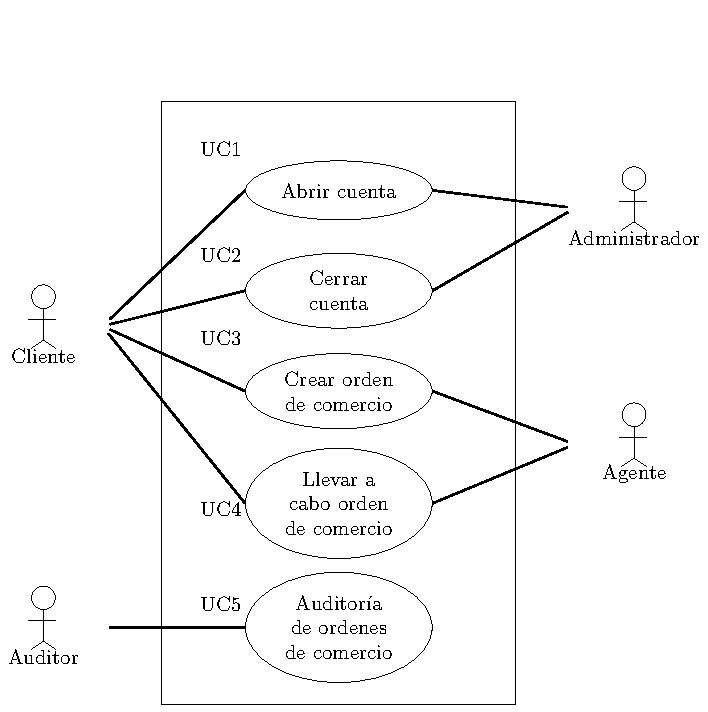
\includegraphics[scale=0.6]{Imagenes/diag_useCase_financialSystem_esp.eps}
    \caption{Casos de uso del sistema financiero.}
    \label{useCases_ex}
\end{figure}


\begin{figure}[hpt!]
\begin{center}
   	\subfloat[Abrir cuenta]{ \label{CU1}
    		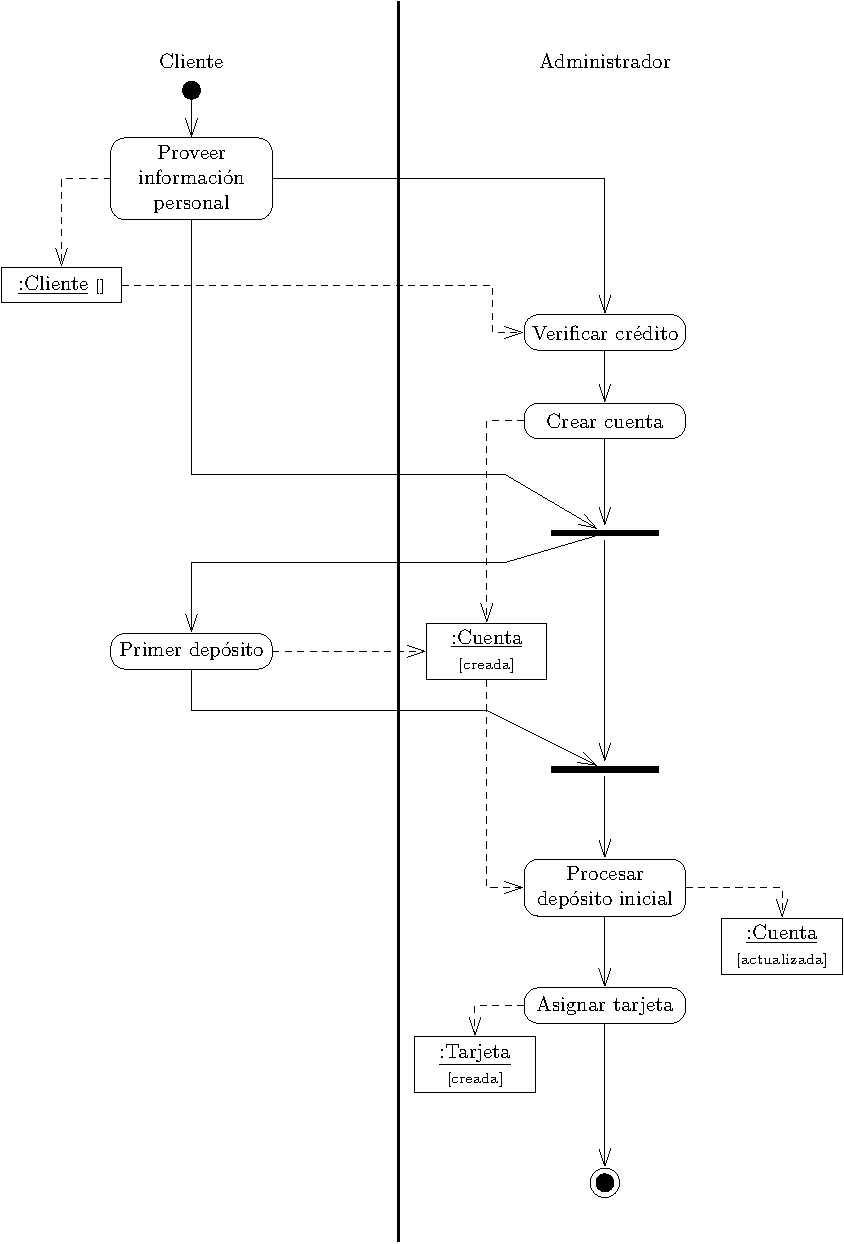
\includegraphics[scale=0.4]{Imagenes/diag_activity_openAccount_esp.eps}}
    		\hspace{1cm}
  	\subfloat[Cerrar cuenta]{ \label{CU2}
    		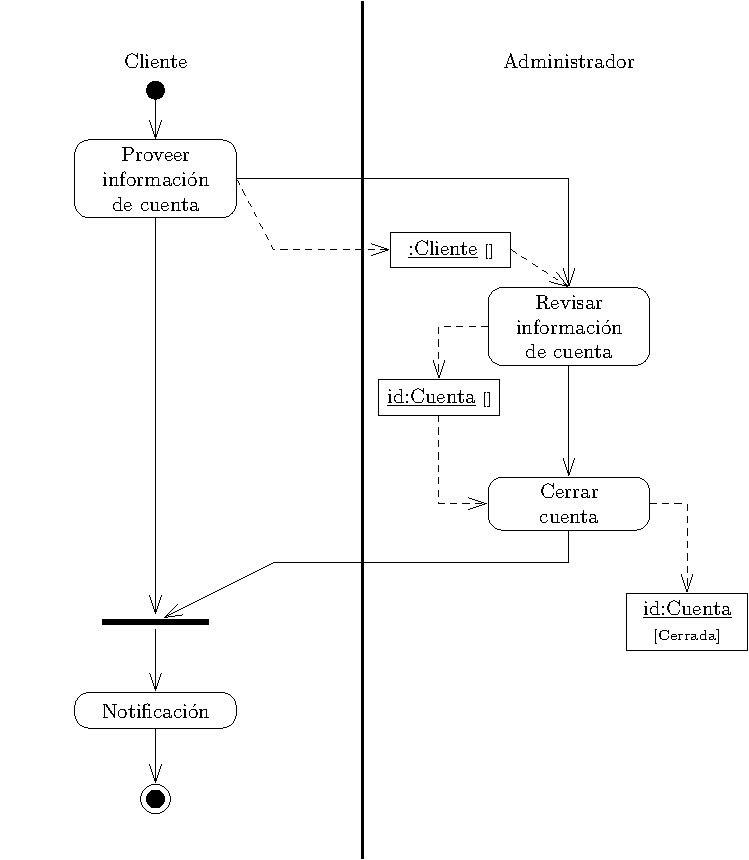
\includegraphics[scale=0.5]{Imagenes/diag_activity_closeAccount_esp.eps}}
 	\caption{Diagramas de actividades parte 1}
 \end{center}
\end{figure}

\begin{figure}[hpt!]
\begin{center}
   	\subfloat[Crear y llevar a cabo orden de comercio]{ \label{CU3y4}
    		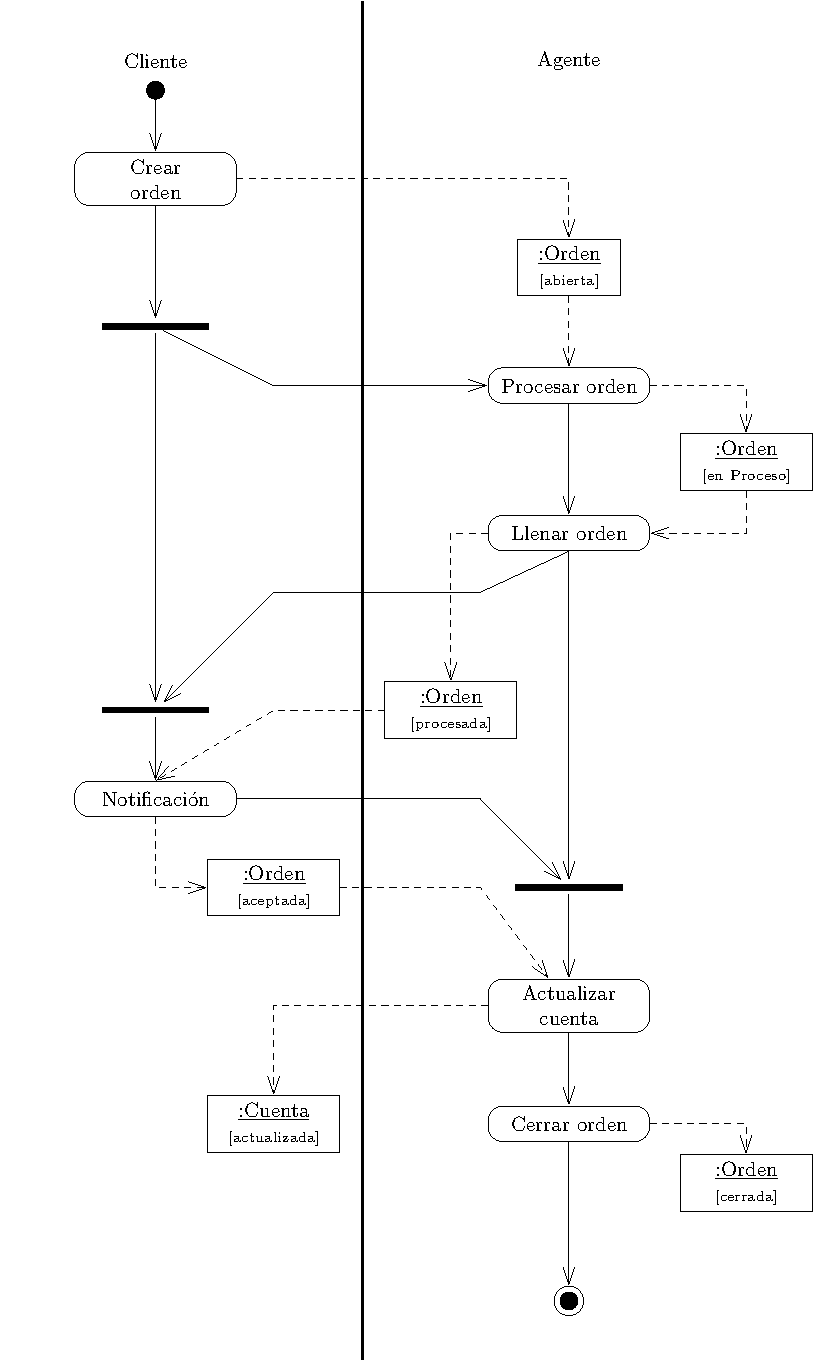
\includegraphics[scale=0.4]{Imagenes/diag_activity_createOrder_esp.eps}}
    		\hspace{1cm}
  	\subfloat[Auditoría de ordenes de comercio]{ \label{CU5}
    		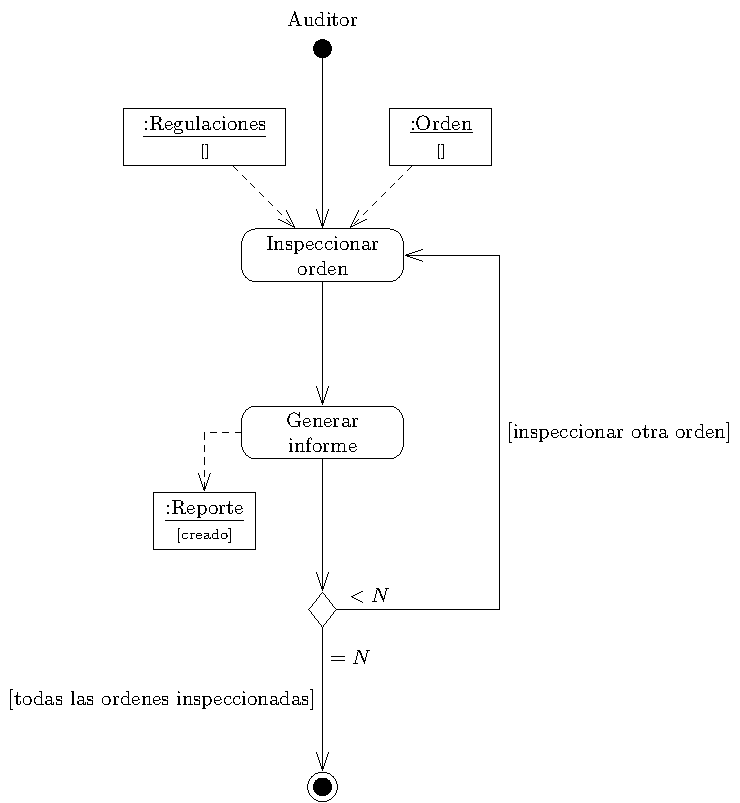
\includegraphics[scale=0.6]{Imagenes/diag_activity_checkTrade_esp.eps}}
 	\caption{Diagramas de actividades parte 2}
 \end{center}
\end{figure}

\subsection{Patrones de seguridad}

La información sobre los patrones de seguridad, patrones de regulación y roles son identificados en el diagrama de clases proporcionado del sistema se muestran de color en la Figura \ref{DC_1}. 

\begin{figure}[p]
  \centering
    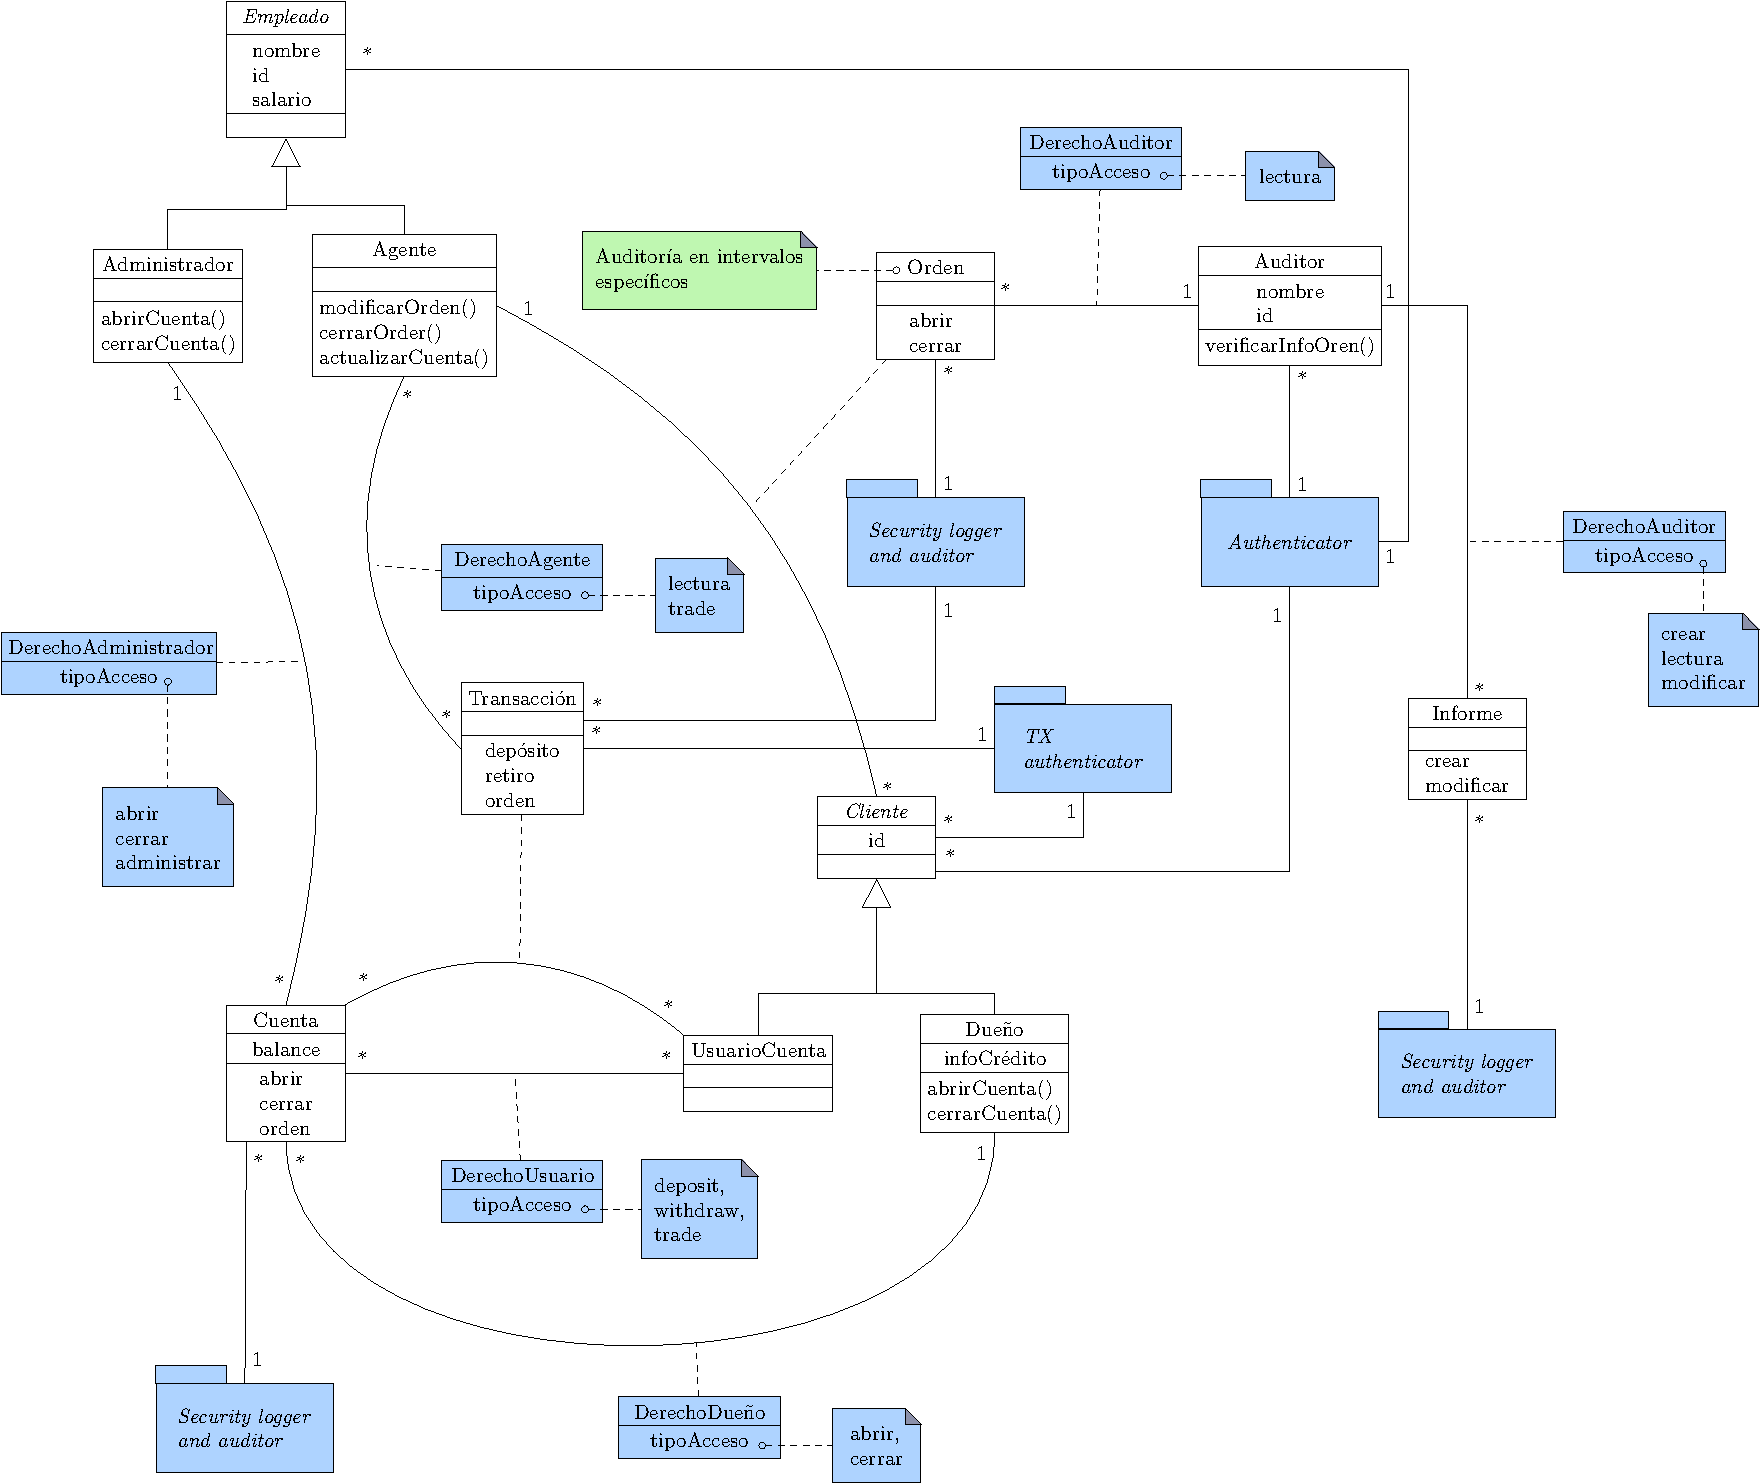
\includegraphics[angle=90,width=\textwidth,height=\textheight]{Imagenes/diag_class_financialSystem_esp.eps}
    \caption{Diagrama de clases de sistema financiero}
    \label{DC_1}
\end{figure}

Los patrones de seguridad aplicados al sistema identificados son:
\begin{enumerate}[noitemsep,label=Pat$_{\arabic*}$:,leftmargin=*]
	\item \textit{Security logger and auditor}
	\item \textit{Role-based access control}
	\item \textit{Authenticator}
	\item \textit{TX Authentication}
\end{enumerate}

Los patrones de regulación identificados en el sistema son:
\begin{enumerate}[noitemsep,label=Reg$_{\arabic*}$:,leftmargin=*]
	\item Realizar auditorías en intervalos específicos.
\end{enumerate}

%Los rolename aplicados al sistema identificados son:
%\begin{enumerate}[noitemsep,label=Rol$_{\arabic*}$:,leftmargin=*]
%	\item 
%\end{enumerate}

\section{Modelado de amenazas}

El análisis de las amenazas sobre los diagramas de actividades se muestra el la Tabla \ref{resFinaSys}. Los diagramas de actividades de mal uso donde se puede observar de manera gráfica el análisis realizado se muestra en las Figuras \ref{CU1_misuse}, \ref{CU2_misuse}, \ref{CU3y4_misuse} y \ref{CU5_misuse}.

\vspace{1cm}

\topcaption{Resultado de amenazas} \label{resFinaSys}
%Primera cabecera - Primera página
\scriptsize{
\tablefirsthead{ 
  \hline 
  \cellcolor{lightgray}\textbf{Actor} &\cellcolor{lightgray} \textbf{Actividad} & \cellcolor{lightgray}\textbf{\#} &\cellcolor{lightgray} \textbf{Atri Seg}&\cellcolor{lightgray}\textbf{Impacto} & \cellcolor{lightgray}\textbf{Origen ataque} &\cellcolor{lightgray} \centering\textbf{Descripción} &\cellcolor{lightgray} \textbf{Activo} \\
}
%Cabecera de páginas subsecuentes
\tablehead{
  \hline
  \multicolumn{8}{|r|}{\tiny Continúa desde la página previa}\\
  \hline
  \cellcolor{lightgray}\textbf{Actor} &\cellcolor{lightgray} \textbf{Actividad} & \cellcolor{lightgray}\textbf{\#} &\cellcolor{lightgray} \textbf{Atri Seg}&\cellcolor{lightgray}\textbf{Impacto} & \cellcolor{lightgray}\textbf{Origen ataque} &\cellcolor{lightgray} \centering\textbf{Descripción} &\cellcolor{lightgray} \textbf{Activo} \\
  \hline
}
%Pie de página de páginas subsecuentes
\tabletail{
  \hline
  \multicolumn{8}{|r|}{\tiny Continúa en la siguiente página}\\
  \hline
}
\tablelasttail{
  \hline
}
\begin{center}
\scriptsize
\setlength{\extrarowheight}{0.4pt}
\begin{mpxtabular}{|P{1cm}|m{1.5cm}|c|P{0.5cm}|c|P{1cm}|m{6cm}|c|}
\hline
	\multicolumn{8}{|c|}{\textit{Abrir cuenta}}\\ \hline
	\multirow{5}{1cm}{Cliente} &\multirow{5}{1.5cm}{Proveer información personal} & T$_{1_1}$ & R & Bajo & InA & Negar haber abierto una cuenta & Cuenta \\ \cline{3-8}
	
	 &  & T$_{1_2}$ & D & Bajo  & Ext & Realizar multiples solicitudes de apertura de cuenta & - \\ \cline{3-8}
	 &  & T$_{1_3}$ & C & Alto & InN/Ext & Leer la información del cliente transmitida por la red  & Cliente \\ \cline{3-8}
	 &  & T$_{1_4}$ & I & Bajo & InA & Provee información inválida (financiera, dirección, etc.)& Cliente \\ \cline{3-8}
	 &  & T$_{1_5}$ & I & Medio & InA & Provee información de otra persona (nombre, dirección, etc.) & Cliente\\ \hline
	 
	 \multirow{5}{1cm}{Gerente} &\multirow{5}{1.5cm}{Verificar historial crediticio} & T$_{2_1}$ & D &Bajo & InA & Negar haber modificado la información crediticia de un cliente & Cliente \\ \cline{3-8}
	
	 &  & T$_{2_2}$     & C & Alto & InA & Recolectar información personal del cliente para distribuirlo ilegalmente & Cliente\\ \cline{3-8}
	 &  & T$_{2_3}$     & C & Alto & InN/Ext & Leer la información del cliente transmitida por la red & Cliente\\ \cline{3-8}
	 &  & T$_{2_4}$ & C & Bajo & Ext & Recolectar información de manera ilegal & Cliente \\ \cline{3-8}
	 &  & T$_{2_5}$ & I & Alto &  InA & Cambiar la información crediticia de un cliente& Cliente  \\ \hline
	 
	  \multirow{4}{1cm}{Gerente} &\multirow{4}{1.5cm}{Crear  cuenta} & T$_{3_1}$ &  R & Bajo & InA& Negar haber creado una cuenta falsa  &  Cuenta \\ \cline{3-8}
	
	 &  & T$_{3_2}$ & C & Alto & InA & Recolectar información de cuentas para distribuirla ilegalmente & Cuenta\\ \cline{3-8}
	 &  & T$_{3_3}$ & C & Medio & InN/Ext  & Leer la información de las cuentas & Cuenta \\ \cline{3-8}
	 &  & T$_{3_4}$ & I & Alto & InA & Crear una cuenta falsa & Cuenta \\ \hline
	 
	 Cliente &Depósito  inicial  &  & - & -&- & &-  \\ \hline
	
	Gerente & Expedir tarjeta& T$_{5_1}$ & I &Alto & InA & Autorizar una tarjeta falsa & Tarjeta \\ \hline
	 
	  \multirow{4}{1cm}{Cliente} &\multirow{4}{1.5cm}{Transferir dinero} & T$_{6_1}$ & R &Medio & InA & Negar haber autorizado una transferencia & Cuenta \\ \cline{3-8}
	 &  & T$_{6_2}$ & D & Bajo & Ext & Inundar a la aplicación de solicitudes de transferencia  & -\\ \cline{3-8}
	 &  & T$_{6_3}$ & C & Bajo & InN/Ext & Leer la información sobre las transferencias del cliente & Cuenta \\ \cline{3-8}
	 &  & T$_{6_4}$ & I &   Alto & Ext & Transferir dinero entre cuentas de manera ilegal & Cuenta \\ \hline
	
	\multicolumn{8}{|c|}{\textit{Cerrar cuenta}}\\ \hline
	\multirow{2}{1cm}{Cliente} &\multirow{2}{1.5cm}{Proveer información personal} & T$_{7_1}$ &R&Bajo&InA&Negar haber solicitado la cancelación de una cuenta&Cuenta \\ \cline{3-8}
	&& T$_{7_2}$ &R&Medio&InN/Ext&Proveer información falsa para solicitar una cancelación de cuenta&Cuenta \\ \hline
	
	Gerente & Revisar cuenta &T$_{8_1}$ & C & Alto &  InN/Ext & Leer la información de la cuenta transmitida por la red & Cuenta  \\ \hline
	
	Gerente & Cerrar cuenta &T$_{9_1}$ & I & Medio &  InA & No cerrar adecuadamente una cuenta para usos ilegales & Cuenta  \\ \hline
	
	
	\multicolumn{8}{|c|}{\textit{Crear y procesar orden de comercio}}\\ \hline
	\multirow{3}{1cm}{Cliente} &\multirow{3}{1.5cm}{Crear orden} & T$_{10_1}$ &I&Medio&InA/Ext&Crear una orden de comercio con información falsa & Orden \\ \cline{3-8}
	&& T$_{10_2}$ &R&Bajo&InA&Negar haber creado una orden de comercio&Orden \\ \cline{3-8}
	&& T$_{10_3}$ &C&Alto&InN/Ext&Leer la información de una orden de comercio transmitida por la red&Orden\\ \hline
	
	\multirow{3}{1cm}{Agente} &\multirow{3}{1.5cm}{Procesar orden} & T$_{11_1}$ &I&Alto&InA&Modificar la información de una orden de comercio & Orden \\ \cline{3-8}
	&& T$_{11_2}$ &R&Alto&InA&Ignorar los reglamentos gubernamentales o de la empresa para procesar una orden &Orden \\ \cline{3-8}
	&& T$_{11_3}$ &R&Bajo&InN&Negar haber procesado una orden de comercio&Orden\\ \hline
	
	Agente &Llevar a cabo orden de comercio & T$_{12_1}$ &I&Alto&InA&Modificar la información de una orden de comercio & Orden \\ \hline
	
	Cliente & Confirmación & - &-&-&-& & - \\ \hline

	Agente&Actualizar cuenta& T$_{14_1}$ &I&Alto&InA/Ext&Transferir el dinero de una orden de comercio a una cuenta de manera ilegal&Cuenta \\ \hline
	
	\multirow{2}{1cm}{Agente} &\multirow{2}{1.5cm}{Cerrar orden} & T$_{15_1}$ &C&Medio&InA&Distribuir información de una orden de comercio de manera ilegal&Orden \\ \cline{3-8}
	&& T$_{15_2}$ &C&Medio&InN/Ext&Leer la información de una orden de comercio&Orden \\ \hline
	
	\multicolumn{8}{|c|}{\textit{Auditoría de ordenes de comercio}}\\ \hline
	

	\multirow{2}{1cm}{Auditor} &\multirow{2}{1.5cm}{Inspeccionar orden} & T$_{16_1}$ &R&Bajo&InA&Negar haber inspeccionado una orden de comercio&Orden \\ \cline{3-8}
	&& T$_{16_2}$ &C&Alto&InA/InN&Copiar información de ordenes para otros usos &Orden \\ \hline
	
	\multirow{3}{1cm}{Auditor} &\multirow{3}{1.5cm}{Generar informe} & T$_{17_1}$ &R&Alto&InA&Ignorar los reglamentos gubernamentales o de la empresa aplicables a una orden al generar el informe &Informe \\ \cline{3-8}
	&& T$_{17_2}$ &R&Medio&InA/InN&Enviar la información de los informes a una persona externa& Informe \\ \cline{3-8}
	&& T$_{17_3}$ &C&Alto&Ext&Leer la información sobre los informes generados& Informe\\ \hline

\end{mpxtabular}
\end{center}
}

\normalsize

\begin{figure}[htp!]
\centering
    	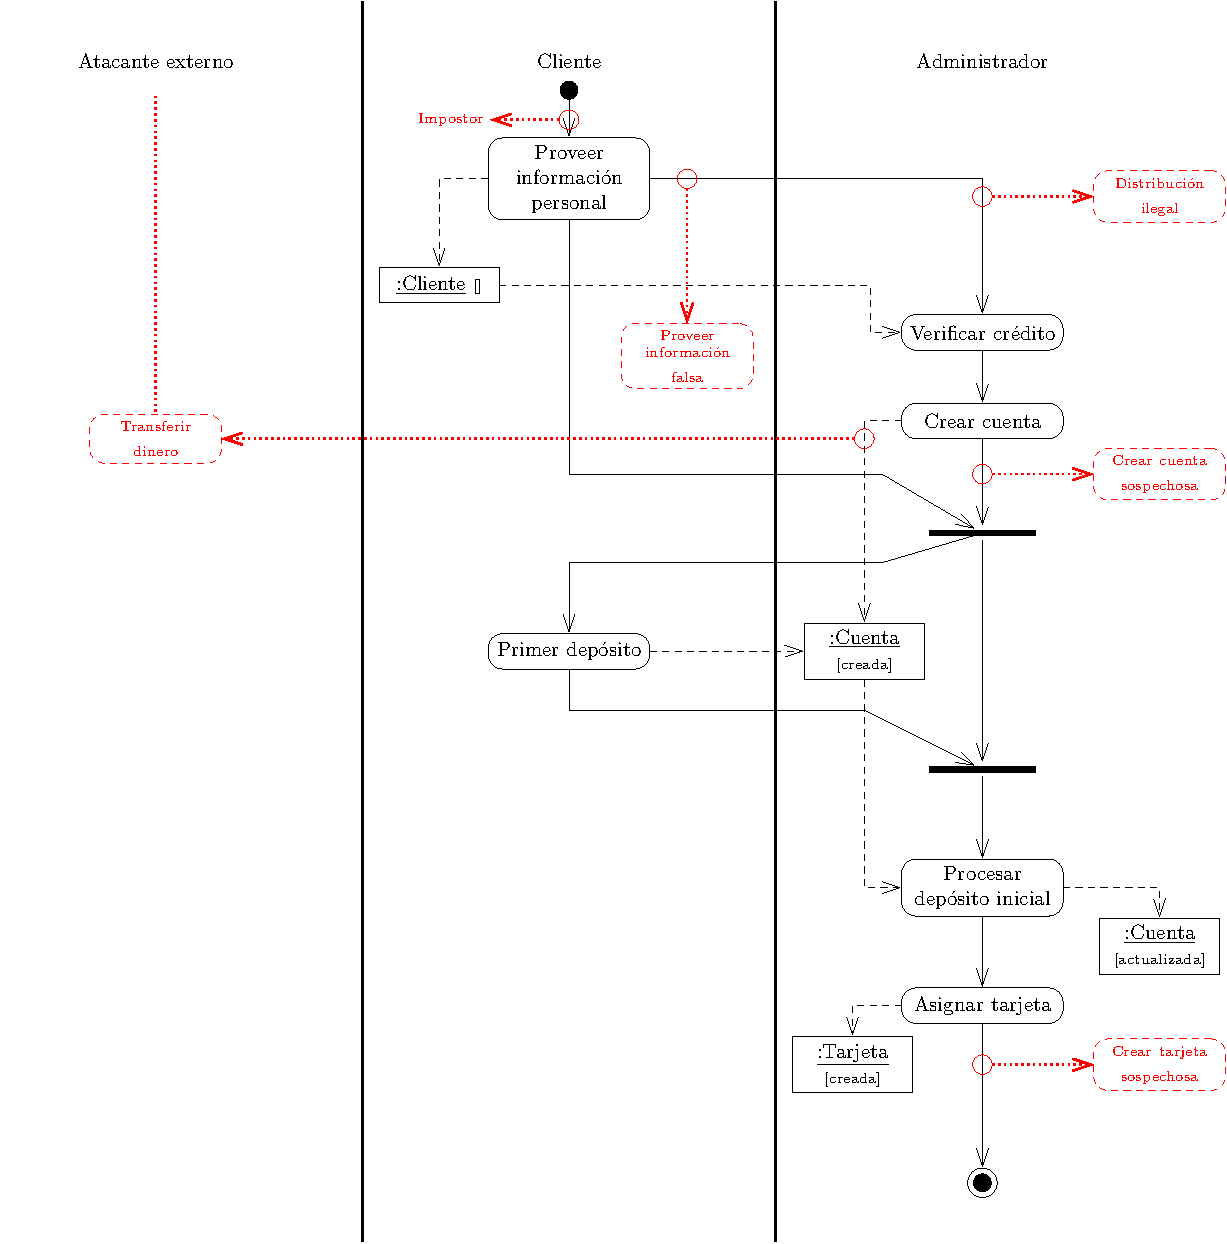
\includegraphics[scale=0.55]{Imagenes/diag_activity_openAccount_misuse_esp.eps}
 	\caption{Diagrama de actividades de mal uso en abrir cuenta}
	\label{CU1_misuse}
\end{figure}

\begin{figure}[htp!]
\centering
    	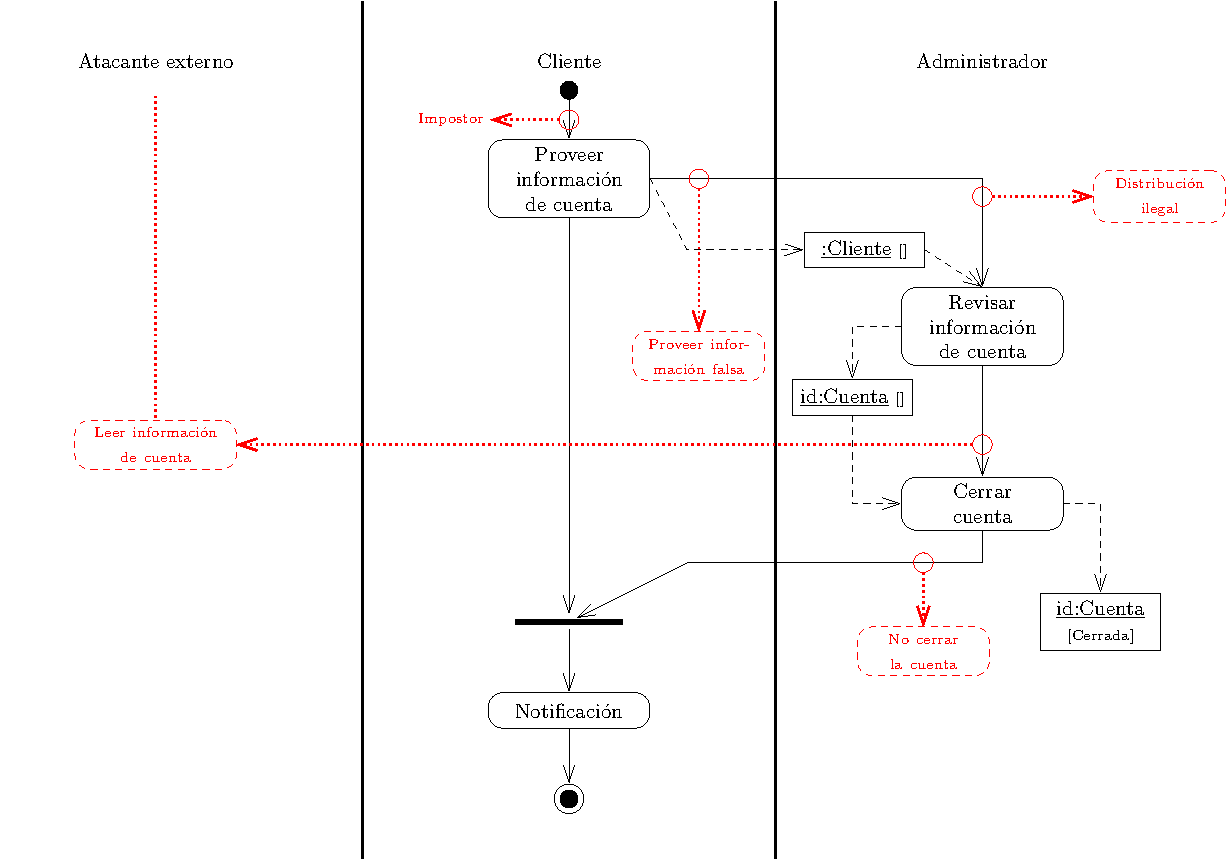
\includegraphics[scale=0.55]{Imagenes/diag_activity_closeAccount_misuse_esp.eps}
 	\caption{Diagrama de actividades de mal uso en cerrar cuenta}
	\label{CU2_misuse}
\end{figure}

\begin{figure}[htp!]
\centering
    	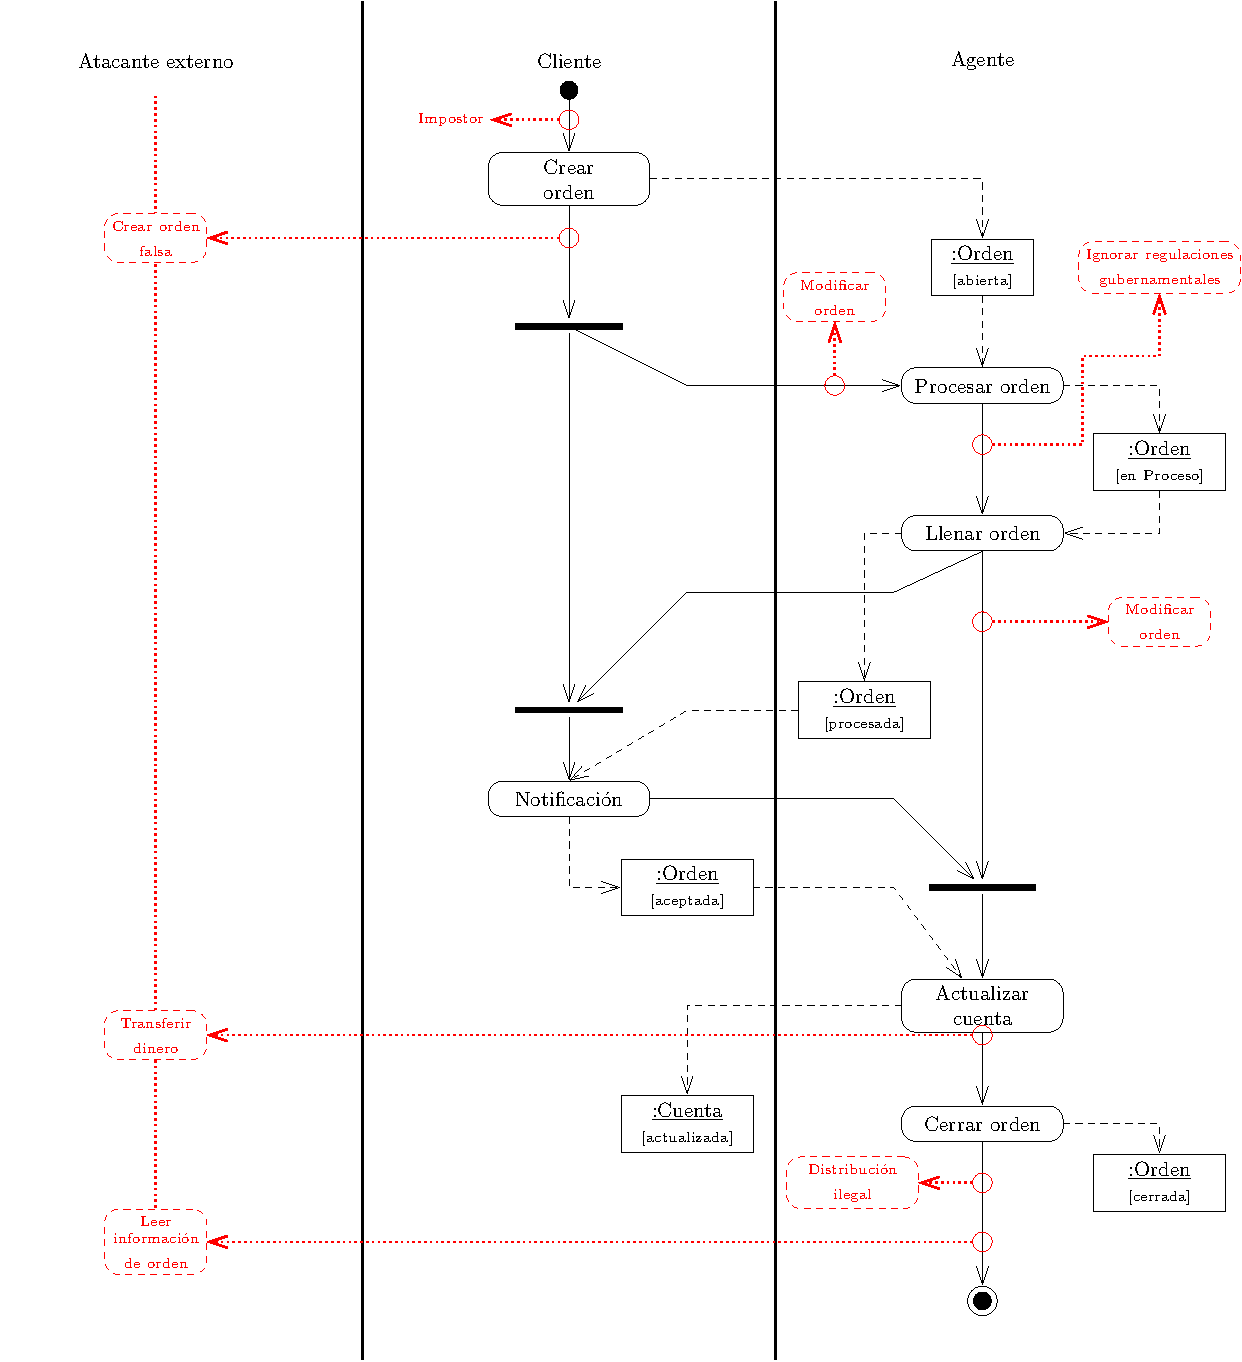
\includegraphics[scale=0.55]{Imagenes/diag_activity_createOrder_misuse_esp.eps}
 	\caption{Diagrama de actividades de mal uso en crear y llevar a cabo orden de comercio}
	\label{CU3y4_misuse}
\end{figure}

\begin{figure}[htp!]
\centering
    	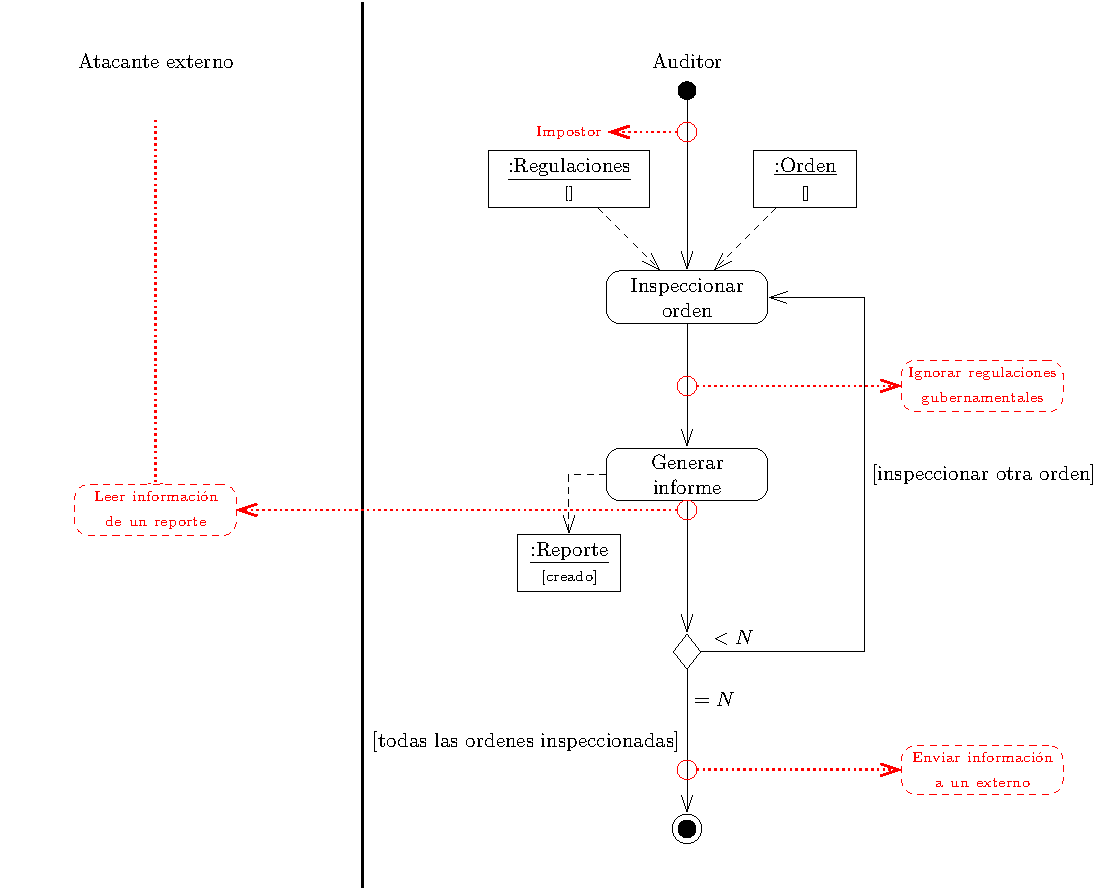
\includegraphics[scale=0.55]{Imagenes/diag_activity_checkTrade_misuse_esp.eps}
 	\caption{Diagrama de actividades de mal uso en auditoría de ordenes de comercio}
	\label{CU5_misuse}
\end{figure}


\section{Evaluación de seguridad del sistema}

\begin{enumerate}[label=Paso \arabic*:,leftmargin=*,noitemsep]
\setcounter{enumi}{0}
	\item Encontrar el peso de las amenazas del sistema $w_{ame}$ con la información contenida en la Tabla \ref{eval_ameSysFinan} plasmando la información como se muestra en la Tabla \ref{eval_ameSysFinan}.
	
	\begin{table}[!ht]
	\caption{Peso de las amenazas mitigadas}
	\renewcommand{\arraystretch}{1.5}
	\begin{center}
	\scriptsize{
	\begin{tabular}{ |c|c|c|c|P{2cm}||c|c|c|c|P{2cm}|}
	\hline
		\cellcolor{lightgray}Amenaza&\cellcolor{lightgray}Patrón(es)&\cellcolor{lightgray}$\alpha$& \cellcolor{lightgray}$v_p$ & \cellcolor{lightgray}$w_{ame}$&\cellcolor{lightgray}Amenaza&\cellcolor{lightgray}Patrón(es)&\cellcolor{lightgray}$\alpha$& \cellcolor{lightgray}$v_p$ & \cellcolor{lightgray}$w_{ame}$ \\ \hline
		T$_{1_1}$&Pat$_1$,Pat$_2$&$\frac{1}{37}$&1&\multirow{19}{*}{}&T$_{7_1}$&Pat$_2$,Pat$_3$,Pat$_4$&$\frac{1}{37}$&1&\multirow{19}{*}{$\frac{\frac{67}{37}}{\frac{81}{37}}=\frac{61}{81}=0.82$}\\\cline{1-4} \cline{6-9}
		T$_{1_2}$&&$\frac{1}{37}$&0&&T$_{7_2}$&Pat$_2$&$\frac{2}{37}$&1&\\ \cline{1-4} \cline{6-9}
		T$_{1_3}$&&$\frac{3}{37}$&0&&T$_{8_1}$&&$\frac{3}{37}$&0&\\\cline{1-4} \cline{6-9}
		T$_{1_4}$&Pat$_2$&$\frac{1}{37}$&1&&T$_{9_1}$&Pat$_3$&$\frac{2}{37}$&1&\\\cline{1-4}\cline{6-9}
		T$_{1_5}$&Pat$_2$&$\frac{2}{37}$&1&&T$_{10_1}$&Pat$_2$,Pat$_3$&$\frac{2}{37}$&1&\\\cline{1-4}\cline{6-9}
		T$_{2_1}$&Pat$_1$,Pat$_2$&$\frac{1}{37}$&1&&T$_{10_2}$&Pat$_3$&$\frac{1}{37}$&1&\\\cline{1-4}\cline{6-9}
		T$_{2_2}$&Pat$_1$&$\frac{3}{37}$&1&&T$_{10_3}$&&$\frac{3}{37}$&0&\\\cline{1-4}\cline{6-9}
		T$_{2_3}$&&$\frac{3}{37}$&0&&T$_{11_1}$&Pat$_1$&$\frac{3}{37}$&1&\\\cline{1-4}\cline{6-9}
		T$_{2_4}$&Pat$_2$&$\frac{1}{37}$&1&&T$_{11_2}$&Pat$_2$,Pat$_3$&$\frac{3}{37}$&1&\\\cline{1-4}\cline{6-9}
		T$_{2_5}$&Pat$_1$&$\frac{3}{37}$&1&&T$_{11_3}$&Pat$_3$&$\frac{1}{37}$&1&\\\cline{1-4}\cline{6-9}
		T$_{3_1}$&Pat$_2$,Pat$_3$&$\frac{1}{37}$&1&&T$_{12_1}$&Pat$_1$&$\frac{3}{37}$&1&\\\cline{1-4}\cline{6-9}
		T$_{3_2}$&Pat$_3$&$\frac{3}{37}$&1&&T$_{14_1}$&Pat$_2$,Pat$_3$,Pat$_4$&$\frac{3}{37}$&1&\\\cline{1-4}\cline{6-9}
		T$_{3_3}$&Pat$_2$&$\frac{2}{37}$&1&&T$_{15_1}$&Pat$_1$,Pat$_2$&$\frac{2}{37}$&1&\\\cline{1-4}\cline{6-9}
		T$_{3_4}$&Pat$_3$&$\frac{3}{37}$&1&&T$_{15_2}$&Pat$_2$&$\frac{2}{37}$&1&\\\cline{1-4}\cline{6-9}
		T$_{5_1}$&Pat$_3$&$\frac{3}{37}$&1&&T$_{16_1}$&Pat$_3$&$\frac{1}{37}$&1&\\\cline{1-4}\cline{6-9}
		T$_{6_1}$&Pat$_2$,Pat$_3$,Pat$_4$&$\frac{2}{37}$&1&&T$_{16_2}$&Pat$_1$&$\frac{3}{37}$&1&\\\cline{1-4}\cline{6-9}
		T$_{6_2}$&&$\frac{1}{37}$&0&&T$_{17_1}$&Pat$_3$&$\frac{3}{37}$&1&\\\cline{1-4}\cline{6-9}
		T$_{6_3}$&Pat$_2$&$\frac{1}{37}$&1&&T$_{17_2}$&Pat$_1$&$\frac{2}{37}$&1&\\\cline{1-4}\cline{6-9}
		T$_{6_4}$&Pat$_4$&$\frac{3}{37}$&1&&T$_{17_3}$&Pat$_2$&$\frac{3}{37}$&1&\\\hline
	\end{tabular}
	}
	\end{center}
	\label{eval_ameSysFinan}
	\end{table}
	\normalsize
	\item Encontrar el peso de los requerimientos de seguridad $w_{req}$ con la información de los requisitos de seguridad y políticas de seguridad encontrados en los previos requeridos. Plasmando la información como se muestra en la Tabla \ref{eval_reqSysFinan}
	
	\begin{table}[!ht]
	\caption{Peso de los requerimientos satisfechos}
	\renewcommand{\arraystretch}{1.5}
	\begin{center}
	\scriptsize{
	\begin{tabular}{ |c|c|c|c|P{2cm}|}
	\hline
		\cellcolor{lightgray}Requisito&\cellcolor{lightgray}Patrón(es)&\cellcolor{lightgray}$\mu$& \cellcolor{lightgray}$v_p$ & \cellcolor{lightgray}$w_{req}$ \\ \hline
		Req$_{1}$&Pat$_1$&$\frac{1}{16}$&1&\multirow{16}{*}{$\frac{\frac{23}{16}}{\frac{42}{16}}=\frac{23}{42}=0.54$}\\ \cline{1-4}
		Req$_{2}$&Pat$_1$&$\frac{3}{16}$&1&\\ \cline{1-4}
		Req$_{3}$&Pat$_2$&$\frac{3}{16}$&1&\\ \cline{1-4}
		Req$_{4}$&Pat$_2$&$\frac{3}{16}$&1&\\ \cline{1-4}
		Req$_{5}$&&$\frac{3}{16}$&0&\\ \cline{1-4}
		Req$_{6}$&Pat$_2$&$\frac{3}{16}$&1&\\ \cline{1-4}
		Req$_{7}$&&$\frac{2}{16}$&0&\\ \cline{1-4}
		Req$_{8}$&&$\frac{3}{16}$&0&\\ \cline{1-4}
		Req$_{9}$&&$\frac{3}{16}$&0&\\ \cline{1-4}
		Req$_{10}$&&$\frac{2}{16}$&0&\\ \cline{1-4}
		Req$_{11}$&Pat$_4$&$\frac{3}{16}$&1&\\ \cline{1-4}
		Pol$_{1}$&&$\frac{3}{16}$&0&\\ \cline{1-4}
		Pol$_{2}$&&$\frac{3}{16}$&0&\\ \cline{1-4}
		Pol$_{3}$&Pat$_2$&$\frac{2}{16}$&1&\\ \cline{1-4}
		Pol$_{4}$&Pat$_3$&$\frac{3}{16}$&1&\\ \cline{1-4}
		Pol$_{5}$&Pat$_2$,Reg$_{1}$&$\frac{2}{16}$&1&\\ \hline
		
	\end{tabular}
	}
	\end{center}
	\label{eval_reqSysFinan}
	\end{table}
	\normalsize
	\item Obtener el valor de la seguridad del sistema con los valores obtenidos del paso anterior. 

	\begin{equation*}
		ss = 0.82 \cdot 0.54 = 0.44
	\end{equation*}
	
\end{enumerate}

\section{Resultado de la evaluación}

Considerando el criterio mostrado en la sección 4.4, el valor obtenido $ss=0.44$ indica que el sistema no se encuentra protegido ante todas las amenazas identificadas y los requisitos de seguridad y/o políticas de seguridad no están siendo satisfechas de manera adecuada. 

\vspace{0.3cm}

Utilizando los valores $w_{ame}$ y $w_{req}$ se identifica la parte del sistema que requiere mejoras. Tomando los valores del ejemplo desarrollado se observa que la parte del sistema que requiere una revisión más exhaustiva por parte de los diseñadores del mismo es la implementación de patrones de seguridad para satisfacer los requisitos de seguridad y políticas de seguridad que se tienen contempladas.

\section{Resumen}

En este capítulo se presenta la evaluación de seguridad de un sistema financiero básico que ejemplifique el método propuesto en el Capítulo 4. En la primera sección se muestra la información del sistema como diagramas UML, requisitos de seguridad y políticas de seguridad. Con la información obtenida de la primera sección, en las secciones posteriores se realiza el análisis de amenazas, la obtención del peso de las amenazas, la obtención del peso de los requisitos de seguridad y por último el resultado de la evaluación. 

\vspace{0.3cm}

La métrica presentada en el presente trabajo muestra la evaluación de seguridad de un sistema que ha sido construido usando patrones de seguridad, analizando la aplicación del método con el ejemplo presentado en este capítulo se plantea la posibilidad de aplicar el método a sistemas que no han sido construidos desde su diseño con patrones de seguridad. 

%El método cambia en la parte de identificar el uso de patrones de seguridad, en lugar de identificarlos en los diagramas UML se identifican en el código del sistema y posteriormente el método se aplica de la misma manera para obtener la evaluación de seguridad.  